
% This LaTeX was auto-generated from MATLAB code.
% To make changes, update the MATLAB code and republish this document.

\documentclass{article}
\usepackage{graphicx}
\usepackage{color}

\sloppy
\definecolor{lightgray}{gray}{0.5}
\setlength{\parindent}{0pt}

\begin{document}

    
    

\section*{16. Best and near-best}

\begin{verbatim}
ATAPformats
\end{verbatim}
\begin{par}
Traditionally, approximation theory has given a great deal of attention to best approximations, by which we continue to mean best approximations in the $\infty$-norm, and rather less to alternatives such as Chebyshev interpolants.  One might think that this is because best approximations are much better than the alternatives. However, this is not true.
\end{par} \vspace{1em}
\begin{par}
In a moment we shall continue with Lebesgue constants to shed some light on this matter, but first, let us do some experiments.  We start with the extreme case of a very smooth function, $\exp(x)$, and compare convergence of its Chebyshev interpolants $p$ and best approximants $p^*$.  (The difference between $n$ and $n+1$ in this code is intentional, since \texttt{chebfun} takes as argument the number of interpolation points whereas \texttt{remez} takes the degree of the polynomial.)
\end{par} \vspace{1em}
\begin{par}
 \vskip -2em 
\end{par} \vspace{1em}
\begin{verbatim}
x = chebfun('x'); f = exp(x); nn = 0:15;
errbest = []; errcheb = []; i = 0;
for n = nn
    i = i+1;
    [p,err] = remez(f,n);
    errbest(i) = err;
    errcheb(i) = norm(f-chebfun(f,n+1),inf);
end
hold off, semilogy(nn,errcheb,'.-r')
hold on, semilogy(nn,errbest,'h-b','markersize',6)
FS = 'fontsize';
text(7,3e-12,'||f-p_n^*||',FS,12)
text(9,2e-7,'||f-p_n||',FS,12)
ylim([1e-16 10])
xlabel n, ylabel error
title(['Convergence of best approximation '...
       'vs. Chebyshev interpolation: exp(x)'],FS,9)
\end{verbatim}

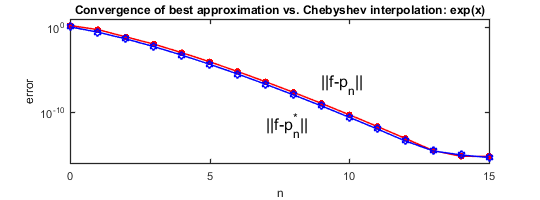
\includegraphics [width=4in]{chap16_01.png}
\begin{par}
 \vskip 1pt 
\end{par} \vspace{1em}
\begin{par}
Clearly the stars for $p^*$ aren't much better than the dots for $p$. The ratio of the two converges toward 2 until the rounding errors set in for larger degrees:
\end{par} \vspace{1em}
\begin{par}
 \vskip -2em 
\end{par} \vspace{1em}
\begin{verbatim}
format short
ratio = errcheb./errbest;
disp('       n       ratio')
fprintf('%8d %12.5f\n',[nn; ratio])
\end{verbatim}

        \color{lightgray} \begin{verbatim}       n       ratio
       0      1.46212
       1      2.00000
       2      1.74436
       3      1.96807
       4      1.94991
       5      1.98188
       6      1.98182
       7      1.98861
       8      1.99105
       9      1.99222
      10      1.99473
      11      1.99161
      12      1.96718
      13      1.10183
      14      0.69390
      15      1.36834
\end{verbatim} \color{black}
    \begin{par}
At the other extreme of smoothness, consider $|x|$:
\end{par} \vspace{1em}
\begin{par}
 \vskip -2em 
\end{par} \vspace{1em}
\begin{verbatim}
f = abs(x); nn = [0 2 4 10 20 40 100 200];
errbest = []; errcheb = []; i = 0;
for n = nn
    i = i+1;
    [p,err] = remez(f,n);
    errbest(i) = err;
    errcheb(i) = norm(f-chebfun(f,n+1),inf);
end
hold off, loglog(nn+1,errbest,'h-b','markersize',6)
hold on, loglog(nn+1,errcheb,'.-r')
axis([1 300 .001 2])
text(5,.01,'||f-p_n^*||',FS,12)
text(26,.06,'||f-p_n||',FS,12)
xlabel n, ylabel error
title(['Convergence of best approximation '...
       'vs. Chebyshev interpolation: |x|'],FS,9)
\end{verbatim}

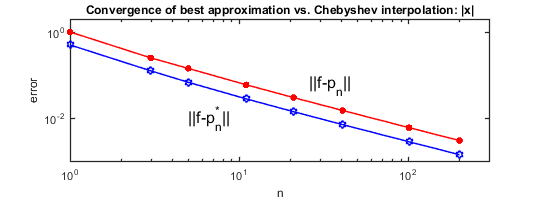
\includegraphics [width=4in]{chap16_02.png}
\begin{par}
 \vskip 1pt 
\end{par} \vspace{1em}
\begin{par}
Again the stars are only a little bit better than the dots, by a constant factor of about 2.13060:
\end{par} \vspace{1em}
\begin{par}
 \vskip -2em 
\end{par} \vspace{1em}
\begin{verbatim}
ratio = errcheb./errbest;
disp('       n       ratio')
fprintf('%8d %12.5f\n',[nn; ratio])
\end{verbatim}

        \color{lightgray} \begin{verbatim}       n       ratio
       0      2.00000
       2      2.00000
       4      2.10234
      10      2.12677
      20      2.12968
      40      2.13037
     100      2.13056
     200      2.13059
\end{verbatim} \color{black}
    \begin{par}
(For odd values of $n$ the ratio is somewhat larger, approaching a constant of about 3.57.)
\end{par} \vspace{1em}
\begin{par}
So for these examples at least, you don't buy much with best approximations.  And the cost in computing time is considerable. Here is the time for computing a Chebyshev interpolant $p$ of degree 200 and evaluating it at 100 points:
\end{par} \vspace{1em}
\begin{par}
 \vskip -2em 
\end{par} \vspace{1em}
\begin{verbatim}
xx = rand(100,1);
tic, p = chebfun(f,201); p(xx); toc
\end{verbatim}

        \color{lightgray} \begin{verbatim}Elapsed time is 0.022605 seconds.
\end{verbatim} \color{black}
    \begin{par}
Here is the time for finding the best approximation $p^*$ and evaluating it at the same points:
\end{par} \vspace{1em}
\begin{par}
 \vskip -2em 
\end{par} \vspace{1em}
\begin{verbatim}
tic, p = remez(f,200); p(xx); toc
\end{verbatim}

        \color{lightgray} \begin{verbatim}Elapsed time is 0.623394 seconds.
\end{verbatim} \color{black}
    \begin{par}
The reason computing $p^*$ is more difficult is that the mapping from $f$ to $p^*$ is nonlinear, hence requiring iteration in a numerical implementation, whereas the mapping from $f$ to $p$ is linear (Exercise 10.5). It is perfectly feasible to compute $p$ for degrees in the millions, whereas for $p^*$ we would rarely attempt degrees higher than hundreds.
\end{par} \vspace{1em}
\begin{par}
Why has $p^*$ received so much more attention than $p$ over the years? One reason is that in the days before fast computers, the degrees were low, so small differences in accuracy were more important. Another is that the theory of best approximations is so beautiful! Indeed, their very nonlinearity makes best approximations seemingly a richer field for research than the simpler Chebyshev interpolants. Everybody remembers Theorem 10.1, the equioscillation theorem, from the moment they first see it.
\end{par} \vspace{1em}
\begin{par}
Yet in actual computation, true best approximations are not so often used, as we have mentioned earlier (Chapter 10). This is a clue that the world of practice may have its own wisdom, independent of the theorists.
\end{par} \vspace{1em}
\begin{par}

Now let us see what theoretical results might tell us about the
difference between $p$ and $p^*$.  The first such results pertain to
Theorems 7.2 and 8.2 given earlier.  Those theorems concerned convergence
rates of $p_n$ to $f$, depending on the smoothness of $f$.  What about
analogous theorems for $p_n^*$?  Apart from constant factors, they turn
out to be the same!  For example, exactly the same bound (8.3) was
published by de la $\hbox{Vall\'ee}$ Poussin [1919, $\hbox{pp.\
123--124],}$ except with the Chebyshev interpolant $p_n$ replaced by the
best approximation $p_n^*$. So within the two classes of functions
considered in Chapters 7 and 8---$f$ having a $k$th derivative of
bounded variation, or $f$ being analytic---there is no clear reason to
expect $p_n^*$ to be much better than $p_n$.

\end{par} \vspace{1em}
\begin{par}
An observation for arbitrary functions $f$ is the following consequence of Theorems 15.1--15.3:
\end{par} \vspace{1em}
\begin{par}
 \em
{\bf Theorem 16.1. Chebyshev projections and interpolants are near-best.}
Let $f\in C([-1,1])$ have degree $n$
Chebyshev projection $f_n$, Chebyshev interpolant
$p_n$, and best approximant $p_n^*$, $n\ge 1$.  Then
$$ \| f-f_n\| \le \left(4 + {4\over \pi^2}\log (n+1)\right)\|f-p_n^*\|
\eqno (16.1) $$
and
$$ \| f-p_n\| \le \left(2 + {2\over \pi} \log (n+1)\right)\|f-p_n^*\|.
\eqno (16.2) $$
\vspace{-1em} 
\end{par} \vspace{1em}
\begin{par}
\textit{Proof.} Follows from Theorems 15.1, 15.2, and 15.3. $~\hbox{\vrule width 2.5pt depth 2.5 pt height 3.5 pt}$
\end{par} \vspace{1em}
\begin{par}
So the loss of accuracy in going from $p_n^*$ to $p_n$, say, can never be larger than a factor of $2 + (2/\pi)\log (n+1)$.  It is interesting to examine the size of this quantity for various values of $n$.  For $n=10^5$, for example:
\end{par} \vspace{1em}
\begin{par}
 \vskip -2em 
\end{par} \vspace{1em}
\begin{verbatim}
2 + (2/pi)*log(100001)
\end{verbatim}

        \color{lightgray} \begin{verbatim}ans =
    9.3294
\end{verbatim} \color{black}
    \begin{par}
Since this number is less than 10, we see that in dealing with polynomials of degree up to $n=100000$, the non-optimality of Chebyshev interpolation can never cost us more than one digit of accuracy.  Here is the computation for $n = 10^{66}$:
\end{par} \vspace{1em}
\begin{par}
 \vskip -2em 
\end{par} \vspace{1em}
\begin{verbatim}
2 + (2/pi)*log(1e66)
\end{verbatim}

        \color{lightgray} \begin{verbatim}ans =
   98.7475
\end{verbatim} \color{black}
    \begin{par}
So we never lose more than 2 digits for degrees all the way up to $10^{66}$---which might as well be $\infty$ for practical purposes. (For British audiences, one can give a talk on these matters with the title `` $\kern -3pt 10^{66}$ and All That''.)
\end{par} \vspace{1em}
\begin{par}
In fact, one might question whether best approximations are really better than near-best ones at all.  Of course they are better in a literal sense, as measured in the $\infty$-norm. However, consider the following error curves, which are quite typical for high degree approximation of a function that is smoother in some regions than others.
\end{par} \vspace{1em}
\begin{par}
 \vskip -2em 
\end{par} \vspace{1em}
\begin{verbatim}
f = abs(x-0.8);
tic, pbest = remez(f,100); toc
hold off, plot(f-pbest,'r')
tic, pcheb = chebfun(f,101); toc
hold on, plot(f-pcheb)
axis([-1 1 -.008 .008]), grid on
title('Best approximation (equiripple) vs. Chebyshev interpolation (spike)',FS,9)
\end{verbatim}

        \color{lightgray} \begin{verbatim}Elapsed time is 0.325320 seconds.
Elapsed time is 0.004672 seconds.
\end{verbatim} \color{black}
    
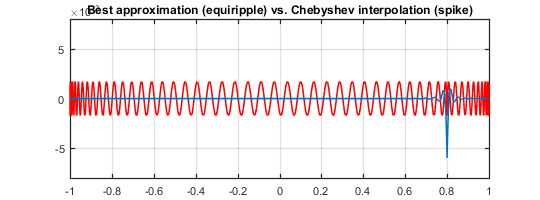
\includegraphics [width=4in]{chap16_03.png}
\begin{par}
 \vskip 1pt 
\end{par} \vspace{1em}
\begin{par}
We see that \texttt{pbest} is worse than \texttt{pcheb} for almost all values of $x$, because the damage done by the singularity at $x=0.8$ is global. By contrast, the effect of the singularity on \texttt{pcheb} decays with distance. Of course, \texttt{pbest} is better in the $\infty$-norm:
\end{par} \vspace{1em}
\begin{par}
 \vskip -2em 
\end{par} \vspace{1em}
\begin{verbatim}
errcheb = norm(f-pcheb,inf)
errbest = norm(f-pbest,inf)
\end{verbatim}

        \color{lightgray} \begin{verbatim}errcheb =
    0.0060
errbest =
    0.0017
\end{verbatim} \color{black}
    \begin{par}
In the 2-norm, however, it is a good deal worse:
\end{par} \vspace{1em}
\begin{par}
 \vskip -2em 
\end{par} \vspace{1em}
\begin{verbatim}
errcheb2 = norm(f-pcheb,2)
errbest2 = norm(f-pbest,2)
\end{verbatim}

        \color{lightgray} \begin{verbatim}errcheb2 =
   4.3337e-04
errbest2 =
    0.0017
\end{verbatim} \color{black}
    \begin{par}
One might question how many applications there might be in which \texttt{pbest} was truly better than \texttt{pcheb} as an approximation to this function $f$.  To echo a title of Corless and Watt [2004], minimax approximations are optimal, but Chebyshev interpolants may sometimes be better!
\end{par} \vspace{1em}
\begin{par}
Li [2004] takes another angle on the near-optimality of Chebyshev interpolants, pointing out that for applications to elementary functions, bounds on certain derivatives usually hold that imply that the error in interpolation in Chebyshev points of the first kind exceeds that of the best approximation by less than a factor of 2, or as he calls it, ``a fractional bit.''
\end{par} \vspace{1em}
\begin{par}
From a more theoretical point of view, we return to a notion mentioned in Theorem 12.1.  Given $f\in C([-1,1])$, let $\rho$ $(1\le \rho \le \infty)$ be the parameter of the largest Bernstein ellipse $E_\rho$ to which $f$ can be analytically continued, and let $\{\kern .5pt p_n\}$ be any sequence of approximations to $f$ with $p_n\in {\cal P}_n$.  Then $$ \limsup_{n\to\infty} \|f-p_n\|^{1/n} \ge \rho^{-1}, $$ and if equality holds, $\{\kern .5pt p_n\}$ is said to be \textit{maximally convergent.}  It follows from Theorem 15.1 that if $\{\kern .5pt p_n\}$ come from a linear projection with Lebesgue constants $\Lambda_n$ that grow more slowly than exponentially as $n\to\infty$, i.e., with $\limsup_{n\to\infty} \Lambda_n^{1/n} = 1$, then $\{\kern .5pt p_n\}$ is maximally convergent for every $f\in C([-1,1])$. In particular, Chebyshev projections and interpolants are maximally convergent.  This is a precise sense in which such approximations are ``near-best''.
\end{par} \vspace{1em}
\begin{par}
Finally, we mention another kind of optimality that has received attention in the approximation theory literature [Bernstein 1931, $\hbox{Erd\H os}$ 1961, Kilgore 1978, de Boor \& Pinkus 1978]: \textit{optimal interpolation points} (Exercise 15.5). Chebyshev points are very good, but they do not quite minimize the Lebesgue constant. Optimal points minimize the Lebesgue constant (by definition), and they level out the peaks of the Lebesgue function exactly (it has been proved)---but the improvement is negligible. The first statement of Theorem 15.2 establishes that, like Chebyshev points, they lead to Lebesgue constants that are asymptotic to $(2/\pi)\log n$ as $n\to\infty$, which means they do not even improve upon Chebyshev points by a constant factor.
\end{par} \vspace{1em}
\begin{par}

\begin{displaymath}
\framebox[4.7in][c]{\parbox{4.5in}{\vspace{2pt}\sl
{\sc Summary of Chapter 16.}
The $\infty$-norm error in degree $n$ Chebyshev interpolation is never
greater than $2+(2/\pi)\log(n+1)$ times the $\infty$-norm error in
degree $n$ best approximation, and in practice, the ratio of errors
rarely exceeds even a factor of\/ $2$.\ \ In the $2$-norm, the
interpolant is often much better than the best approximation.
\vspace{2pt}}}
\end{displaymath}

\end{par} \vspace{1em}
\begin{par}
 \small\smallskip\parskip=2pt
{\bf Exercise 16.1. Computing times for interpolation
and best approximation.}
(a) Repeat the experiment of this chapter involving $|x-0.8|$ but for all
the values $n = 100, 200, 300, \dots ,1000$.  In each case measure the
computing times for Chebyshev interpolation and best approximation as
calculated by the Chebfun {\tt remez} command, the
$L^2$ errors of both approximants, and the $L^\infty$ errors.  Plot these
results and comment on what you find.  (b) In particular, produce a plot
of error curves like that in the text.  You may find it helpful to use a
flag like {\tt 'numpts',10000} in your Chebfun plotting command.
\par
{\bf Exercise 16.2.  Approximation of a wiggly function.}
Define $f(x) = T_{200}(x)+T_{201}(x) + \cdots + T_{220}(x)$.
Construct the Chebyshev interpolant $p$ and best approximation
$p^*$ of degree 199.  Plot the errors and measure the
$\infty$- and $2$-norms.
\par
{\bf Exercise 16.3.  Rounding errors on a grid of \boldmath$10^{66}$ points.}
Suppose we had a computer with 16-digit precision capable of applying the
barycentric formula (5.13) to evaluate a polynomial interpolant $p(x)$ for
data on a Chebyshev
grid of $10^{66}$ points. (For the sake of this thought experiment, imagine
that the differences $x-x_j$ can be evaluated correctly to $16$-digit precision
rather than coming out as $0$ and thereby invoking the
$x=x_j$ clause of Theorem 5.2.)
The evaluation would require adding up about $10^{66}$ numbers, entailing
about $10^{66}$ rounding errors.  Even if these errors only accumulated
in the square root fashion of a random walk, it would still
seem we must end up with errors on the order of $10^{33}$ times
$10^{-16}$, destroying all accuracy.  Yet in fact, the computation would
be highly accurate.  What is the flaw in this $10^{33}$ reasoning?
\par 
\end{par} \vspace{1em}



\end{document}
    
